\section{Applikation}                                   
I følgende afsnit gøres der rede for beslutningerne i forhold til udvikling af applikationens styresystem.

\subsection{Styresystem}
Der findes mange forskellige styresystemer i dag. De to brugte er dog iOS \cite{iOS} og Android. \cite{Android} \\
IOS er Apples eget styresystem som er udviklet i forhold til deres mobile og tablet devices. \\
Android er et stort open source project som bliver brugt på ca. 80\% af alle mobile og tablet devices i dag. Der findes forskellige versioner af Android styresystemet alt efter hvilken producent der har leveret devices. \\
De mest kendte Android device leverendører er firmaer som Samsung, Huawei og HTC. De har alle en Android Core i deres styresystemer, men har alle også videre udviklet styresystemet, så det passer specifikt til deres devices.

Rambøll ønskede en applikation udviklet til iOS. Til en workshop med Rambøll, fandt vi ud af at der også var ansatte som bruger Android. Derfor blev der aftalt at udvikle cross-platform. \\

\subsection{Cross-platform udviklingsværktøjer}
I denne sektion vil der være en kort beskrivelse af nogle cross-platform udviklingsværktøjer.

\subsubsection{Xarmarin}
Xarmarin tilbyder en cross-platform, hvor der udviklet i C\#\cite{CSharp} og XAML\cite{XAML}.
Features Xarmarin tilbyder:
\begin{itemize}[-]
	\item Integreret i Visual Studio
	\item API Access 
	\item Deling af kode
\end{itemize}

\subsubsection{PhoneGap}
PhoneGap er en platform udviklet af Adobe\cite{Adobe}. Her bruges teknologier som HTML5\cite{HTML5}, JavaScripts\cite{JavaScript} og CSS\cite{CSS}. \\
Deres platform tilbyder nogle bonus features som:
\begin{itemize}[-]
	\item Build server
	\item Easy share af applikationen 
	\item Mulitple plug-ins
\end{itemize}

\subsubsection{Corona}
Corona tilbyder en cross-platform, hvor der udviklet i Lua scripting \cite{Lua}.
\begin{itemize}[-]
	\item Real time simulering
	\item Live testing
	\item Mange Plug-in muligheder
	\item Gratis at bruge
\end{itemize}

\subsubsection{Sencha}
Sencha er en platform som er baseret på web applikations udvikling. De bruger teknologier som ES6\cite{ES6}, HTML5\cite{HTML5}, JavaScripts\cite{JavaScript} og CSS\cite{CSS}. \\
Deres platform tilbyder en masse ekstra ved hjælp af Ext JS frameworket. Nogle af disse er f.eks:
\begin{itemize}[-]
	\item Pre-integrerede og testede UI komponenter
	\item Data visualisering
	\item Back-end Data package
	\item Layout Manager
\end{itemize}


\subsection{Valg af cross-platform udviklingsværktøj}
Da der skulle bestemmes hvilken cross-platform der skulle arbejdes med, var der ikke meget tvivl. \\
Der var et lille kendskab til Xarmarin fra et tidligere projekt lavet på Ingeniør Højskolen. \\
Xarmarin giver mulighed for at skrive i C\# som er et sprog der er blevet undervist i på skolen og er et højniveau sprog. \\
Xarmarin blev i februar 2016 opkøbt af Microsoft, hvilket betyder at det siden da har været en integreret del af Microsoft Visual Studio, som er det fortrukne udviklingsværktøj.\\
Developer dokumentationen for Xarmarin er også et plus. Hvis man sidder med et problem, har Xarmarin lavet en meget grundig dokumentation, hvor man kan finde eksempler og guides til hvordan forskellige dele i en applikaiton skal programmeres.

\subsection{Xarmarin}
I denne sektion vil der komme en mere dybdegående beskrivelse af hvordan Xarmarin platformen er bygget op.



\begin{figure}[H]
	\centering
	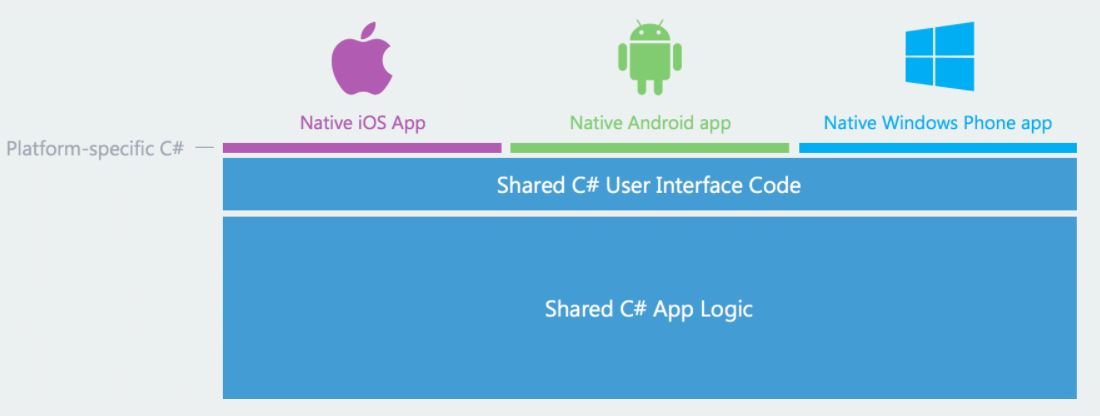
\includegraphics[width=1\linewidth]{Applikation/XarmarinShare.JPG}
	\caption{Kode deling i Xarmarin}
	\label{fig:CodeShare}
\end{figure}


\clearpage